%%%%%%%%%%%%%%%%%%%%%%%%%%%%% Define Article %%%%%%%%%%%%%%%%%%%%%%%%%%%%%%%%%%
\documentclass{article}
%%%%%%%%%%%%%%%%%%%%%%%%%%%%%%%%%%%%%%%%%%%%%%%%%%%%%%%%%%%%%%%%%%%%%%%%%%%%%%%

%%%%%%%%%%%%%%%%%%%%%%%%%%%%% Using Packages %%%%%%%%%%%%%%%%%%%%%%%%%%%%%%%%%%
\usepackage{listings, xcolor}
\usepackage{parskip}
\usepackage{hyperref}
\usepackage{amsmath}
\usepackage{graphicx}
\usepackage[a4paper, margin = 1.5cm]{geometry}
\usepackage{float}
\usepackage{amsmath}
\usepackage{amssymb}
\usepackage{parskip}
\usepackage{listings}

\lstset{
frame = shadowbox,
basicstyle = \small\ttfamily,
mathescape = true,
numbers = left,
commentstyle = \itshape\color{gray}
columns = flexible,
keepspaces = true,
moredelim = [l]{//}
}

%%%%%%%%%%%%%%%%%%%%%%%%%%%%%% Title & Author %%%%%%%%%%%%%%%%%%%%%%%%%%%%%%%%
\title{Testing Black Box e White Box}
\author{Trentin Tommaso}
%%%%%%%%%%%%%%%%%%%%%%%%%%%%%%%%%%%%%%%%%%%%%%%%%%%%%%%%%%%%%%%%%%%%%%%%%%%%%%
\begin{document}
\maketitle
\tableofcontents
\newpage

  \section{Testing black box}
    Sistema appare come una "scatola nera" (struttura interna non visibile al tester), approccio particolarmente utile quando non si ha accesso a codice sorgente. Consiste nell'esercitare il sistea immettendo input e osservando valori degli outut.
    \begin{itemize}
        \item Sfrutta conoscenza di:
          \begin{itemize}
              \item Interfaccia del sistema;
              \item Documentazone (es. descrizione degli scenari).
          \end{itemize}
        \item Non tiene conto di:
          \begin{itemize}
              \item Codice sorgente;
              \item Stato interno dell'applicazione.
          \end{itemize}
    \end{itemize}
    Gli obiettivi principali del testing black box possono essere la \textit{copertura degli scenari di esecuzione} definiti nei casi d'uso o la \textit{copertura delle funzionalità} definite nella specifica dei requisiti, tuttavia lo spazio dei possibili input è estremamente ampio e ne va quindi scelto un sottoinsieme significativo.
    \subsection{Classi di equivalenza}
      In base ai requisiti dei SW richiesto si suddivide lo spazio degli input in sottoinsiemi detti \textbf{classi di equivalenza} i cui elementi (idealmente) si comporteranno allo stesso modo durante l'esecuzione. I casi di test eseguiranno poi \textit{almeno un test per ogni classe di equivalenza}.
      \subsubsection{Suddivisione}
        Anche spazio dell'output può essere diviso in partizioni di equivalenza in cui il sistema avrà comportamento simile. Si può considerare la caratteristica di \textbf{validità} dell'input a esercitare una particolare funzionalità del SW per definire 1+ classi di \textbf{input validi} e 1+ di \textbf{input non validi}.
    \subsection{Boundary values}
      Programmatori fanno spesso errori per valori di input vicini ai confini (boundaries) delle classi di equivalenza. Il SW va quindi testato anche con valori di input che coincidono (o sono vicini) ai valori limite delle classi di equivalenza.
      \subsubsection{Problemi}
        A volte non è possibile determinare a priori input per coprire le classi di equivalenza ma bisogna comunque conoscere le precondizioni, in tal caso va specificata la \textbf{precondizione} in modo da tenere conto di quali valori per le variabili sono accettabili.
  \section{Testing white box}
    Utilizza struttura interna del SW per ricavare dati di test, può fornire maggiori info al debugger sulla posizione dell'errore e complementa il testing black box in quanto controlla le parti di programma non testate da esso che potrebbero contenere errori.
    \begin{figure}[htpb]
        \centering
        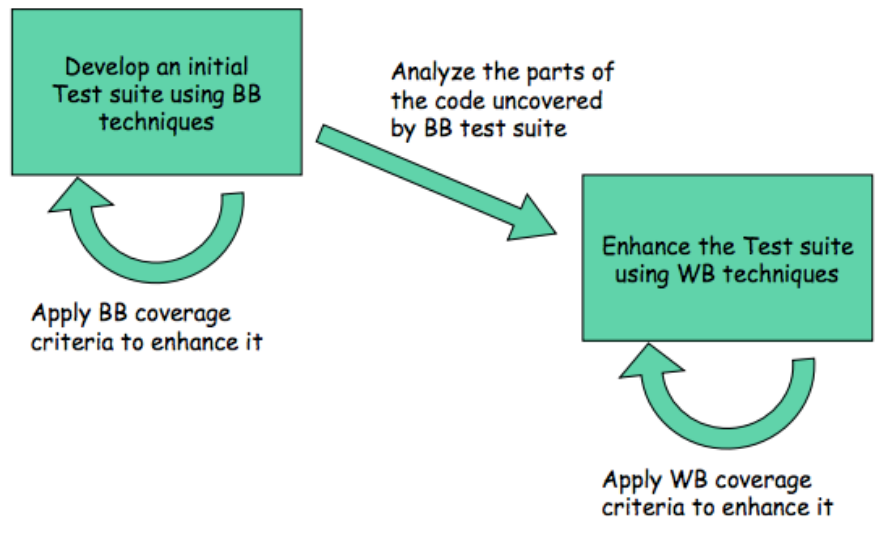
\includegraphics[width=0.6\linewidth]{figures/bb_wb.png}
    \end{figure}
  \section{Control Flow Graph (CFG)}
    \subsection{Idea}
      \noindent
        \begin{minipage}[c]{0.58\linewidth}
            Grafo orientato che rappresenta il trasferimento del flusso di controllo tra blocchi di istruzioni di un programma P, contiene:
            \begin{itemize}
                \item \textbf{nodi} che rappresentano blocchi di 1+ istruzioni, tutte eseguite se il flusso di controllo raggiunge la prima di esse;
                \item \textbf{archi} che rappresentano trasferimento del flusso di controllo tra coppia di nodi che esso collega;
                \item \textbf{nodo di ingresso} e \textbf{nodo d'uscita}
            \end{itemize}
            I nodi possono essere:
            \begin{itemize}
                \item \textbf{istruzione} con 1 solo arco uscente;
                \item \textbf{predicato} che corrispondono a condizioni e hanno 2 archi uscenti corrispondenti a V/F o 3+ archi uscenti in caso di switch-case.
            \end{itemize}
        \end{minipage}
        \hfill
        \begin{minipage}[c]{0.38\linewidth}
            \centering
            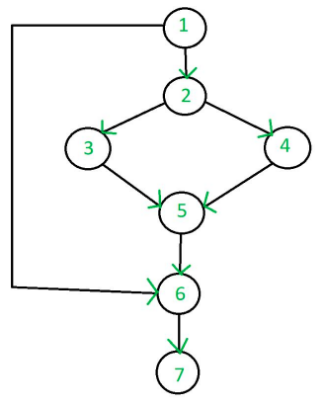
\includegraphics[width=0.7\linewidth]{figures/cfg.png}
        \end{minipage}
      \subsubsection{Nodi predicato}
        \begin{figure}[htpb]
            \centering
            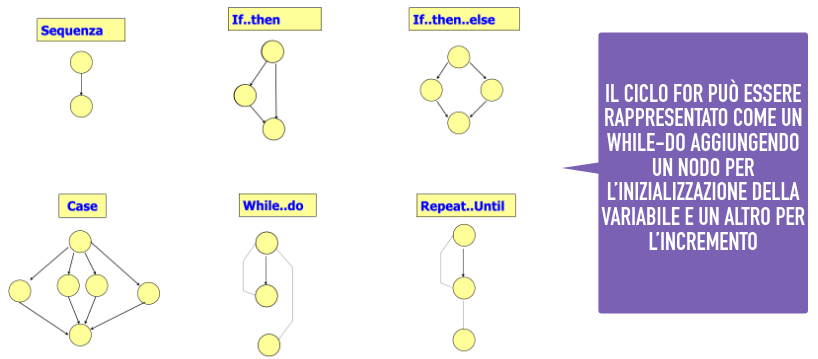
\includegraphics[width=0.7\linewidth]{figures/nod_pre.png}
        \end{figure}
      \subsubsection{Code to CFG}
        \begin{figure}[htpb]
            \centering
            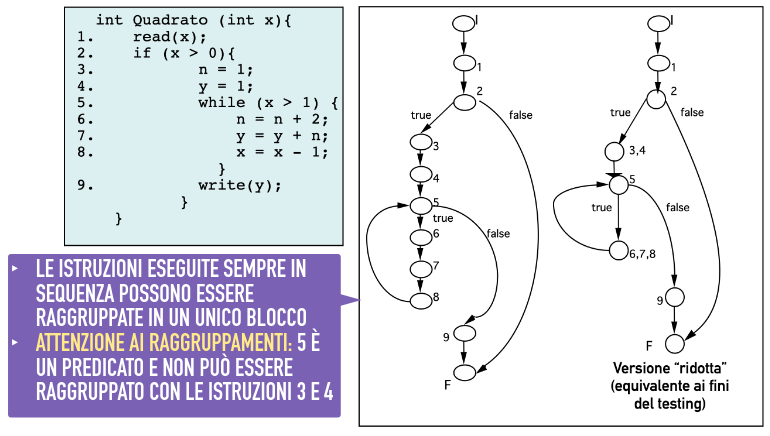
\includegraphics[width=0.6\linewidth]{figures/co_cfg.png}
        \end{figure}
    \subsection{Criteri di copertura}
      Fondati sull'adozione di metodi di Coperturaa degli oggetti che compongono struttura dei programmi, vanno definiti un insieme di casi di test aventi dati in input in grado di \textbf{coprire} tutti i componenti di interesse del SW almeno una volta durante la loro esecuzione.
      \subsubsection{Copertura dei comandi (Statement coverage)}
        \noindent
          \begin{minipage}[c]{0.58\linewidth}
              Richiede di coprire tutti i nodi del CFG durante il testing ed eseguire tutte le istruzioni, il che dà una debole garanzia di scoprire i difetti essendo abbastanza semplice da soddisfare (non assicura di coprire sia il ramo \textit{true} che il ramo \textit{false} delle decisioni).
          \end{minipage}
          \hfill
          \begin{minipage}[c]{0.38\linewidth}
              \centering
              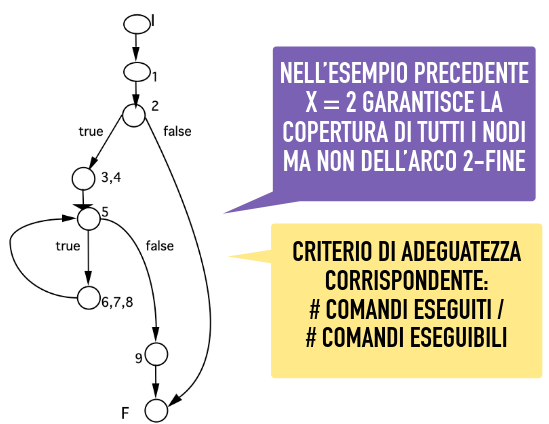
\includegraphics[width=0.7\linewidth]{figures/sta_cov.png}
          \end{minipage}
      \subsubsection{Copertura delle decisioni (Decision coverage)}
        \noindent
          \begin{minipage}[c]{0.58\linewidth}
              Richiede che ciascun arco del CFG sia attraversato almeno una volta, ogni decisione del programma deve quindi assumere sia valore \textit{true} che valore \textit{false} durante il testing. Unico limite in caso di decisioni in cui vengono valutate più condizioni.
          \end{minipage}
          \hfill
          \begin{minipage}[c]{0.38\linewidth}
              \centering
              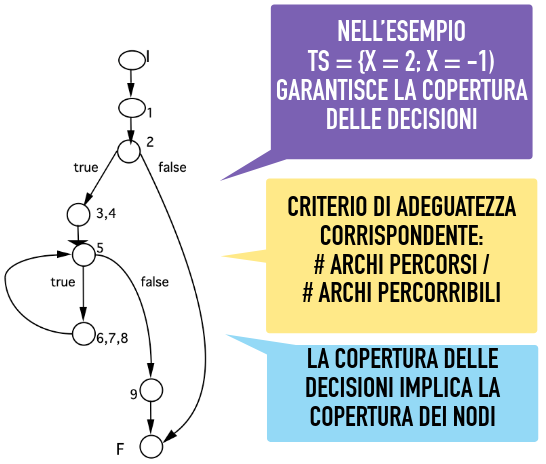
\includegraphics[width=0.7\linewidth]{figures/dec_cov.png}
          \end{minipage}
      \subsubsection{Decisioni vs condizioni}
        \begin{itemize}
            \item \textbf{Decisione}: predicato di una istruzione confizionale o di una iterativa;
            \item \textbf{Condizione}: espressione atomica booleana che appare in una decisione.
        \end{itemize}
        \begin{figure}[htpb]
            \centering
            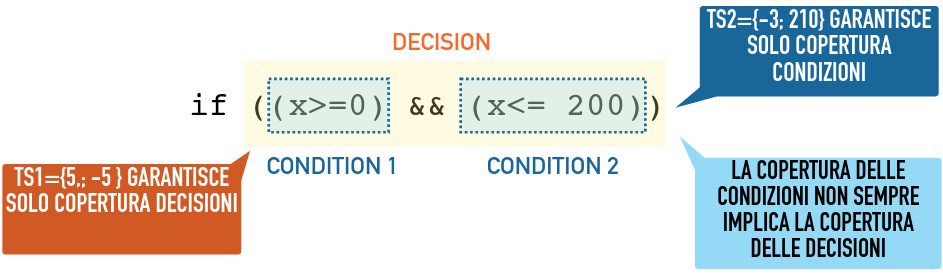
\includegraphics[width=0.8\linewidth]{figures/dec_cond.png}
        \end{figure}
      \subsubsection{Condition coverage}
        Richiede che ciascuna condizione dei nodi decisione di un CFG debba essere valutata per valori sia \textit{true} che \textit{false}.
      \subsubsection{Copertura di condizioni E decisioni}
        Criterio più forte perché assicura che casi di test coprono tutte le condizioni ma anche tutte le decisioni.
        \begin{figure}[htpb]
            \centering
            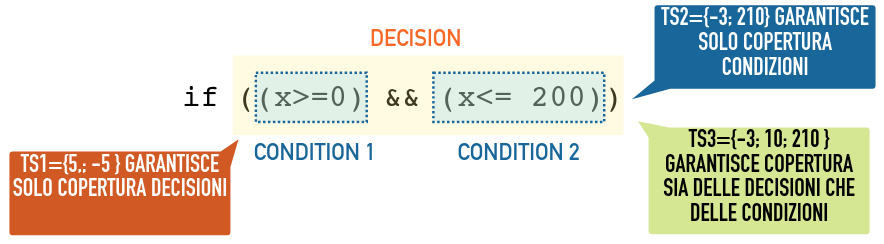
\includegraphics[width=0.8\linewidth]{figures/dec_cond_cov.png}
        \end{figure}
    \subsection{Esempio}
      \begin{center}
          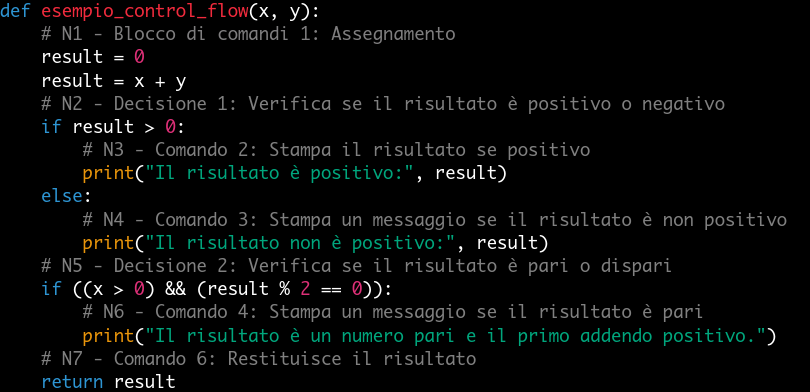
\includegraphics[width=0.8\linewidth]{figures/cov_es_1.png}
      \end{center}
      \vspace{1cm}
      \noindent
        \begin{minipage}[c]{0.48\linewidth}
            \centering
            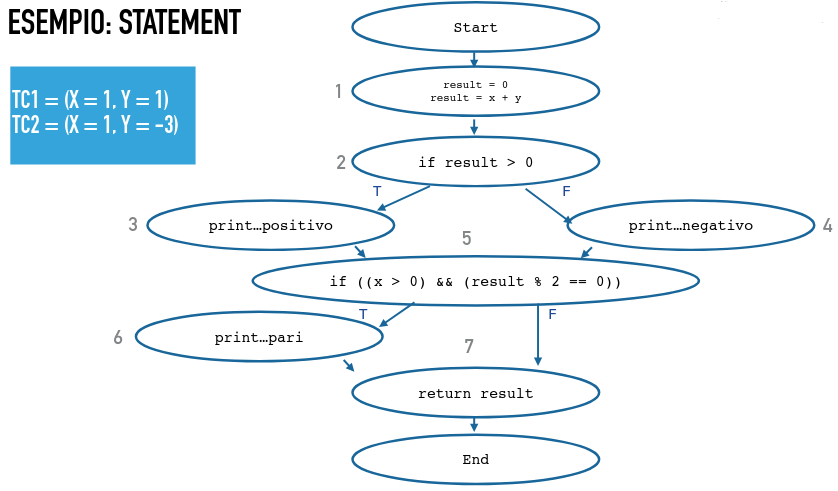
\includegraphics[width=0.9\linewidth]{figures/cov_es_2.png}
        \end{minipage}
        \hfill
        \begin{minipage}[c]{0.48\linewidth}
            \centering
            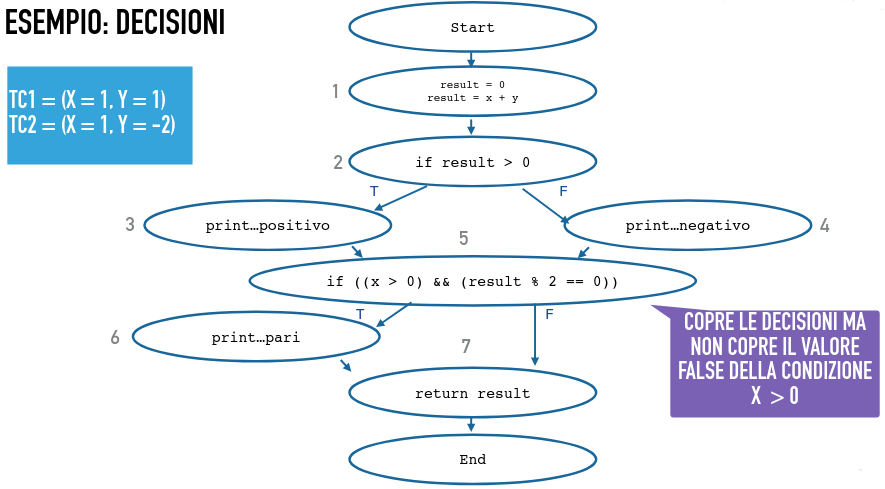
\includegraphics[width=0.9\linewidth]{figures/cov_es_3.png}
        \end{minipage}
      \noindent
        \begin{minipage}[c]{0.48\linewidth}
            \centering
            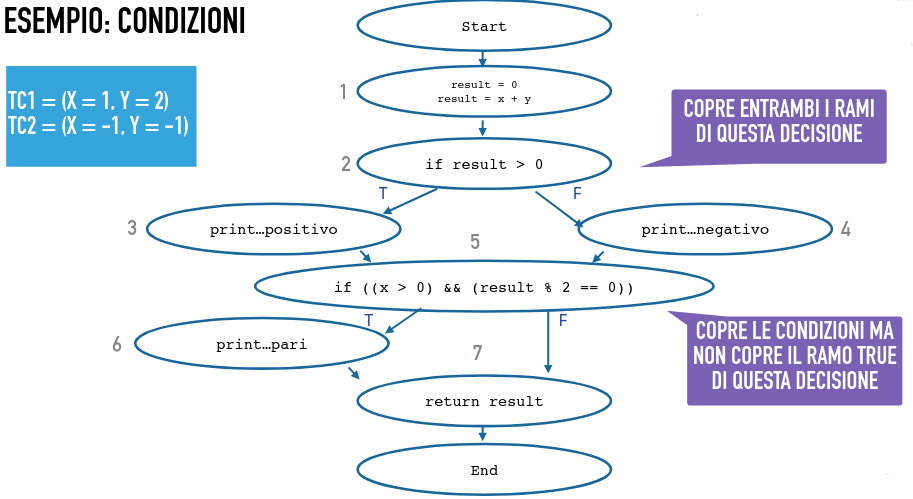
\includegraphics[width=0.9\linewidth]{figures/cov_es_4.png}
        \end{minipage}
        \hfill
        \begin{minipage}[c]{0.48\linewidth}
            \centering
            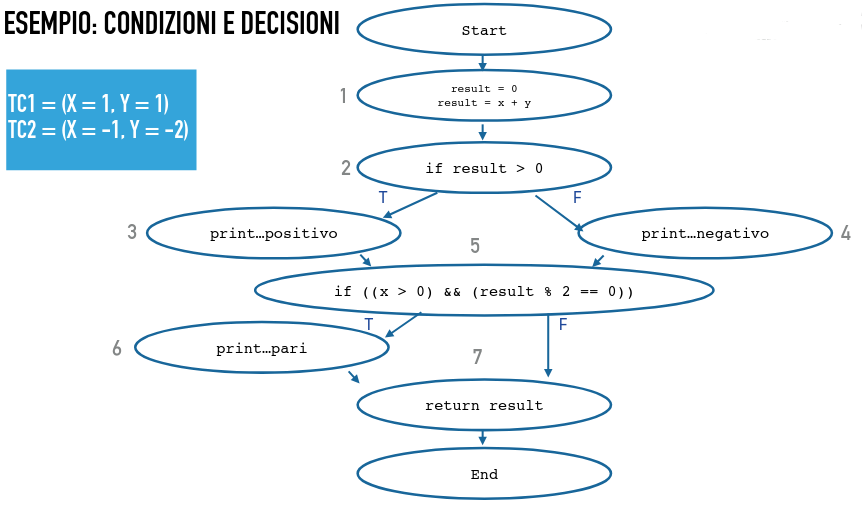
\includegraphics[width=0.9\linewidth]{figures/cov_es_5.png}
        \end{minipage}
\end{document}

